\documentclass[12pt]{article}
\usepackage[UTF8]{ctex}
\usepackage{xeCJK}
\usepackage[margin=1in]{geometry}
\usepackage{graphicx} % For including figures
\usepackage{amsmath}  % For math fonts, symbols and environments
\usepackage{pgfgantt} % For Gantt charts
\usepackage[hidelinks]{hyperref} % For hyperlinks
\usepackage{enumitem} % For customizing lists
\definecolor{blue}{HTML}{74BBC9}
\definecolor{yellow}{HTML}{F7E967}
\usepackage{listings}
\usepackage{xcolor}
\usepackage{tocloft} % 导入tocloft包
\usepackage{zi4}
\usepackage{fontspec}
\usepackage{setspace} % For setting line spacing

\usepackage{booktabs} % For professional looking tables
\usepackage{array}    % For extended column definitions
\usepackage{amsfonts} % For math fonts like '\mathbb{}'
\usepackage{amssymb}  % For math symbols
\usepackage{caption}  % For custom captions
\usepackage[table]{xcolor} % For coloring tables
\usepackage{tabularx} % For auto-sized table columns
\usepackage{algorithm}

\usepackage{algpseudocode}
\usepackage{enumitem}
\usepackage{tikz}
\usetikzlibrary{positioning}

% 目录标题样式定义
\renewcommand{\cfttoctitlefont}{\hfill\Large\bfseries}
\renewcommand{\cftaftertoctitle}{\hfill\mbox{}\par}

% 设置中文主字体为宋体,指定相对路径
\setCJKmainfont[
    Path = ./fonts/,
    BoldFont = SimSun.ttc,
    ItalicFont = SimSun.ttc
]{SimSun.ttc}

% 设置英文主字体为Times New Roman
\setmainfont{Times New Roman}

% 设置正文格式:宋体,小四,行距20磅
\renewcommand\normalsize{%
    \CJKfamily{song}\fontsize{12pt}{20pt}\selectfont}

% Monokai theme with a lighter background
\definecolor{codegreen}{rgb}{0,0.6,0}
\definecolor{codegray}{rgb}{0.5,0.5,0.5}
\definecolor{codepurple}{rgb}{0.58,0,0.82}
\definecolor{backcolour}{rgb}{0.95,0.95,0.92}
\setmonofont{Source Code Pro}[Contextuals={Alternate}]

\lstdefinestyle{mystyle}{
    backgroundcolor=\color{backcolour},   
    commentstyle=\color{codegreen},
    keywordstyle=\color{magenta},
    numberstyle=\tiny\color{codegray},
    stringstyle=\color{codepurple},
    basicstyle=\ttfamily\footnotesize,
    breakatwhitespace=false,         
    breaklines=true,                 
    captionpos=b,                    
    keepspaces=true,                 
    numbers=left,                    
    numbersep=5pt,                  
    showspaces=false,                
    showstringspaces=false,
    showtabs=false,                  
    tabsize=2
}

\lstset{style=mystyle}



\title{\textbf{ML第四次实验报告}}
\author{58122204 谢兴}
\date{\today}

\begin{document}


\begin{titlepage}
  \centering
  \vspace*{60pt}
  \Huge\textbf{机器学习实验报告}

  \vspace{100pt}
  \Large
  实验名称:实现支持向量机

  \vspace{25pt}
  学生:谢兴

  \vspace{25pt}
  学号:58122204

  \vspace{25pt}
  日期:2024/6/1

  \vspace{25pt}
  指导老师:刘胥影

  \vspace{25pt}
  助教:田秋雨



\end{titlepage}


\newpage
\tableofcontents


\section{任务描述}
通过两种方式实现SVM:
\begin{enumerate}
  \item 手动实现SMO算法,并与直接使用传统二次规划方法进行对比。
  \item 通过scikit-learn库实现软间隔SVM。
\end{enumerate}
并在breast cancer数据集上进行验证与实验。该数据集是一个二分类问题,属性均为连续属性,并已进行标准化。


\section{问题复述}
\subsection{手动实现SVM的SMO算法}
SVM的对偶问题实际是一个二次规划问题,除了SMO算法外,传统二次规划方法也可以用于求解对偶问题。求得最优拉格朗日乘子后,
超平面参数$w, b$可由以下式子得到:
\begin{equation}
  \textbf{w} = \sum_{i=1}^{m} \alpha_{i}y_{i}x_{i}
\end{equation}

\begin{equation}
  b=\frac{1}{|S|}\sum_{s\in S}(\frac{1}{y_{s}}-\sum_{s\in S}\alpha_{i}y_{i}\mathbf{x_{i}^{T}x_{s}})
\end{equation}
请完成以下任务:
\begin{enumerate}
  \item 不考虑软间隔情况,直接使用传统二次规划(QP)方法求解(实现)训练集上的硬间隔SVM对偶问题。
        观察并回答,这样的求解方法是否会出现问题,为什么?
  \item 不限定硬间隔或是软间隔SVM,也不限定是否为核化SVM,根据需要选择合适的方法,手动实现SMO算法 求解SVM对偶问题。
        注意第3步,KKT条件验证步骤不能缺少。
  \item 对测试数据进行预测,确保预测结果尽可能准确。
\end{enumerate}

\subsection{使用sklearn库简洁实现软间隔SVM}
\subsubsection{使用sklearn库简洁实现软间隔SVM。首先实现以下4个示例性的SVM模型:}

\begin{enumerate}
  \item 线性SVM:正则化常数C=1,核函数为线性核,
  \item 线性SVM:正则化常数C=1000,核函数为线性核,
  \item 非线性SVM:正则化常数C=1,核函数为多项式核,d=2,
  \item 非线性SVM:正则化常数C=1000,核函数为多项式核,d=2,
\end{enumerate}
观察并比较它们在测试集上的性能表现。

\subsubsection{参数选择与参数分析}
参数的选择对SVM的性能有很大的影响。确定正则化常数C与核函数及其参数的选择范围(可以在以下常用核函数中选择一种或多种),
选用合适的实验评估方法(回顾第2章的内容,如K折交叉验证法等)进行参数选择,并进行参数分析实验。


\begin{enumerate}
  \item

        正则化常数C的选择范围可以是以下数量级,如:\(\{10^{-3}, 10^{-2}, 10^{-1}, 1, 10, 10^2, 10^3\}\)
  \item
        核函数
        \begin{itemize}
          \item 线性核:\(k(x,y) = x^T y\),无参数,退化为SVM基本型
          \item 多项式核:\(k(x,y) = (x^T y + c)^d\)
                \begin{itemize}
                  \item \(c\):偏移量,通常取值0或1
                  \item \(d\):多项式的次数,通常取值2, 3, 4等较小的整数,取值为1时退化为线性核
                \end{itemize}
          \item 多项式核另外一种常用的形式:\(k(x,y) = (\gamma \cdot x^T y + c)^d\)
                \begin{itemize}
                  \item \(\gamma\):用于控制核函数的影响范围,常用值为\(1/\text{n\_features}\),n\_features是属性个数,或者也可以尝试0.001, 0.01, 0.1, 1, 10等
                  \item \(c\):偏移量,通常取值0或1
                  \item \(d\):多项式的次数,通常取值2, 3, 4等较小的整数,取值为1时退化为线性核
                \end{itemize}
          \item 高斯核/RBF核:\(k(x,y) = \exp(-\gamma \|x - y\|^2)\)
                \begin{itemize}
                  \item \(\gamma\):带宽参数,控制核函数的平滑程度。常用取值范围为\(\{10^{-3}-10^3\}\)。典型值为\(1/(\text{n\_features} \cdot X.\text{var}())\),其中\(X.\text{var}()\)表示数据集\(X\)的方差,这可以确保 \(\gamma\) 的值在数据特征的数量和数据的方差范围内适当缩放。
                \end{itemize}
          \item Laplace核:\(k(x,y) = \exp(-\gamma \|x - y\|)\)
                \begin{itemize}
                  \item \(\gamma\):带宽参数,控制核函数的平滑程度。常用取值范围参考高斯核的 \(\gamma\) 值
                \end{itemize}
          \item Sigmoid核函数:\(k(x,y) = \tanh(\gamma \cdot x^T y + c)\)
                \begin{itemize}
                  \item \(\gamma\):缩放因子,常用取值范围为\(\{10^{-3}-10^3\}\)
                  \item \(c\):偏移量,通常取值0或1
                \end{itemize}
        \end{itemize}
\end{enumerate}

请注意,SVM中的参数通常需要联合选择,特别是对于核函数的参数与正则化参数\(C\)。参数联合优化的策略有:
\begin{enumerate}
  \item 网格搜索:网格搜索是一种穷举搜索法,在给定的参数空间中逐一尝试每种可能的参数组合,并选用合适的评估方法进行评估。
  \item 随机搜索:在参数空间中对参数组合的随机采样进行评估。通常可以在较大的参数空间中找到接近最优的参数组合。步骤如下:
        \begin{itemize}
          \item 定义参数的取值范围
          \item 随机采样若干参数组合
          \item 对每个采样的参数组合进行评估
          \item 选择性能最优的参数组合
        \end{itemize}
  \item 贝叶斯优化:贝叶斯优化是一种更为高级的优化方法,通过构建一个模型来估计参数空间的性能分布,并通过最大化预期改进(Expected Improvement, EI)等准则来选择下一组参数进行评估。其步骤如下:
        \begin{itemize}
          \item 初始采样若干参数组合并进行评估
          \item 构建模型(如高斯过程回归)
          \item 基于模型选择下一组参数进行评估
          \item 更新模型并重复第3个步骤,直到达到预定的评估次数或满足停止条件。
        \end{itemize}
\end{enumerate}



本实验中可以选择较为简单的网格搜索策略或随机搜索策略进行调参。

参数分析实验需要报告:

\begin{enumerate}
  \item 评估方法
  \item 参数取值范围
  \item 搜索策略
  \item 比较分析每组参数上的性能情况
  \item 最终选择的最优参数
\end{enumerate}



\section{实验环境}
实验环境见表~\ref{tab:indicators}。

\begin{table}[!t]
  \caption{Experiment Environment}
  \label{tab:indicators}
  \centering
  \begin{tabular}{m{5cm}<{\centering}m{5cm}<{\centering}m{4cm}<{\centering}}
    \toprule
    \textbf{Items}   & \textbf{Version}     \\[\medskipamount]
    \midrule
    CPU              & Intel Core i5-1135G7 \\[\medskipamount]
    RAM              & 16 GB                \\[\medskipamount]
    Python           & 3.11.5               \\[\medskipamount]
    scikit-learn     & 1.3.2                \\[\medskipamount]
    Operating system & Windows11            \\[\medskipamount]
    \bottomrule
  \end{tabular}
\end{table}

\section{实验过程}
\subsection{手动实现SMO算法}

\subsubsection{传统QP算法求解硬间隔SVM的对偶问题}
在本实验中,我们首先使用传统的二次规划(QP)方法求解硬间隔SVM的对偶问题。代码实现的大致思路如下:

具体的实验步骤和结果如下:

\begin{enumerate}
  \item 加载训练数据并求解硬间隔SVM:从CSV文件加载训练数据,调用上述函数求解SVM问题,得到模型参数(权重w和偏置b)。
  \item 定义预测函数:根据训练好的模型参数,对测试数据进行预测。
\end{enumerate}

实验结果如下图~\ref{QP Algorithm for Support Vector Machine} 所示。

\begin{figure}[htbp]
  \centering
  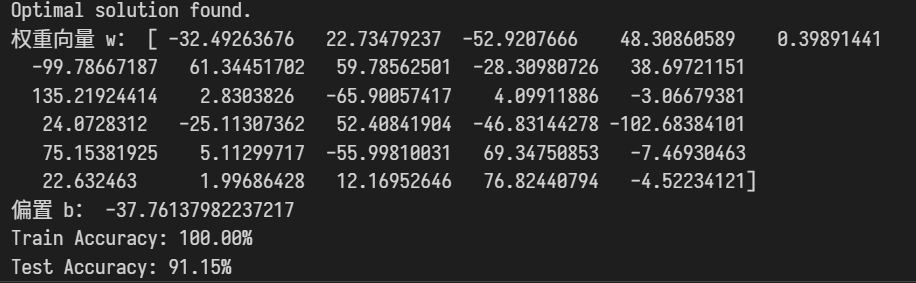
\includegraphics[width=0.5\textwidth]{figures/QP_hard_SVM_result.png}
  \caption{QP Algorithm for Support Vector Machine}
  \label{QP Algorithm for Support Vector Machine}
\end{figure}

从实验结果可以看出,硬间隔SVM的训练准确率达到了100\%,模型能够完美地分类训练数据。在对测试数据进行预测时,模型的准确率也达到了91\%。



\subsubsection{手动实现SMO算法 求解SVM对偶问题}

在本实验中,我们手动实现了SMO算法来求解支持向量机(SVM)的对偶问题。代码实现的大致思路如下:
\begin{enumerate}
  \item 定义核函数:我们使用线性核函数来计算样本之间的内积。
  \item 定义求解QP问题的函数:使用cvxopt库解决二次规划问题,包括创建QP问题的矩阵并求解。
  \item 加载训练数据并求解硬间隔SVM:从CSV文件加载训练数据,调用上述函数求解SVM问题,得到模型参数(权重w和偏置b)。
  \item 定义预测函数:根据训练好的模型参数,对测试数据进行预测。
\end{enumerate}

通过这些步骤,我们成功实现了SMO算法,并求解了SVM的对偶问题,得到了模型的参数(权重w和偏置b)。

\subsubsection{对测试数据进行预测}

在完成模型训练后,我们使用训练得到的模型对测试数据进行了预测。
% 具体的实验步骤和结果如下:
% \begin{enumerate}
%   \item 加载测试数据并进行预测:从CSV文件加载测试数据,调用预测函数进行预测,并计算准确率。
%   \item 保存预测结果并与原始标签进行对比:将预测结果保存到CSV文件中,并与原始标签进行对比,找出不同之处。
% \end{enumerate}

% 实验结果如下图所示:

% \begin{figure}[H]
%   \centering
%   \includegraphics[width=0.5\textwidth]{path_to_accuracy_image}  % 请将此路径替换为您实际的图像路径
%   \caption{测试集准确率}
% \end{figure}

% \begin{figure}[H]
%   \centering
%   \includegraphics[width=0.5\textwidth]{path_to_comparison_image}  % 请将此路径替换为您实际的图像路径
%   \caption{原始标签与预测标签的对比}
% \end{figure}

测试集准确率达到了98.25\%。在对比测试数据中的预测值和原始标签时,我们发现有2处不同。具体不同之处如下表所示:

\begin{table}[h]
  \centering
  \begin{tabular}{ccc}
    \toprule
    样本索引 & 原始标签 & 预测标签 \\
    \midrule
    20   & 1    & -1   \\
    77   & 1    & -1   \\
    \bottomrule
  \end{tabular}
  \caption{原始标签与预测标签的不同之处}
\end{table}

通过这些实验,我们验证了手动实现的SMO算法在解决SVM对偶问题上的有效性,并展示了其在实际数据集上的应用效果。


\subsubsection{QP算法和SMO算法的对比}
从实验结果和上述分析可以看出手动实现的SMO算法要比传统的QP算法更加高效,尤其是在大规模数据集上。
SMO算法通过选择两个变量来优化目标函数,而QP算法需要求解整个拉格朗日乘子向量,
因此在大规模数据集上,SMO算法的计算效率更高。
此外,SMO算法还可以更好地处理非线性核函数,因此在实际应用中更加灵活。


\subsection{使用sklearn库简洁实现软间隔SVM}

\subsubsection{实现4个示范性的SVM模型}

在本实验中,我们使用了sklearn库来实现4个示范性的SVM模型,并在breast cancer数据集上进行训练和测试。这些模型包括:

\begin{enumerate}
  \item 线性SVM:正则化常数C=1,核函数为线性核
  \item 线性SVM:正则化常数C=1000,核函数为线性核
  \item 非线性SVM:正则化常数C=1,核函数为多项式核,d=2
  \item 非线性SVM:正则化常数C=1000,核函数为多项式核,d=2
\end{enumerate}

以下是各个模型在测试集上的性能表现:

\begin{itemize}
  \item \textbf{线性SVM (C=1)}:
        \begin{itemize}
          \item 准确率:0.9825
        \end{itemize}

  \item \textbf{线性SVM (C=1000)}:
        \begin{itemize}
          \item 准确率:0.9561
        \end{itemize}

  \item \textbf{非线性SVM (C=1, d=2)}:
        \begin{itemize}
          \item 准确率:0.9825
        \end{itemize}

  \item \textbf{非线性SVM (C=1000, d=2)}:
        \begin{itemize}
          \item 准确率:0.9386
        \end{itemize}
\end{itemize}

从实验结果可以看出:
\begin{itemize}
  \item 线性SVM在C=1时的表现优于C=1000时的表现,表明适当的正则化有助于提高模型的泛化能力。
  \item 非线性SVM在C=1时的表现优于C=1000时的表现,这与线性SVM的情况相似,说明过大的正则化常数可能导致模型过拟合。
  \item 多项式核SVM(d=2)的表现与线性SVM相当,表明在此数据集上,线性模型已经能够很好地分类数据,复杂的非线性核函数并未显著提升性能。
\end{itemize}


\subsubsection{参数分析实验}

在本实验中,我们进行了参数选择与参数分析。我们选择的参数范围如下:

\begin{itemize}
  \item 正则化常数C的选择范围:\(\{10^{-3}, 10^{-2}, 10^{-1}, 1, 10, 10^2, 10^3\}\)
  \item 核函数:
        \begin{itemize}
          \item 线性核:\(k(x,y) = x^T y\)
          \item 多项式核:\(k(x,y) = (x^T y + c)^d\),其中\(c\)通常取值0或1,\(d\)通常取值2, 3, 4等较小的整数
          \item 高斯核/RBF核:\(k(x,y) = \exp(-\gamma \|x - y\|^2)\),\(\gamma\)的常用取值范围为\(\{10^{-3}到10^3\}\)
          \item Laplace核:\(k(x,y) = \exp(-\gamma \|x - y\|)\),\(\gamma\)的常用取值范围与高斯核相同
          \item Sigmoid核函数:\(k(x,y) = \tanh(\gamma x^T y + c)\),\(\gamma\)的常用取值范围为\(\{10^{-3}到10^3\}\),\(c\)通常取值0或1
        \end{itemize}
  \item 核函数参数:
        \begin{itemize}
          \item 多项式核:度数\(d\)的选择范围:\(\{2, 3, 4\}\)
          \item 高斯核、Laplace核、Sigmoid核:\(\gamma\)的选择范围:\(\{0.001, 0.01, 0.1, 1, 10, 100\}\)
        \end{itemize}
\end{itemize}

我们使用网格搜索(GridSearchCV)方法对以上参数进行了交叉验证(5折交叉验证),最终选择了最佳的参数组合。

\begin{itemize}
  \item \textbf{最佳参数:}\['C': 0.001, 'degree': 2, 'gamma': 0.001, 'kernel': 'linear', 'laplacian\_gamma': 0.001\]
  \item \textbf{最佳交叉验证准确率:}0.9780
\end{itemize}

从实验结果可以看出,线性核函数的表现最佳,同时适当的小的正则化常数C(如0.001)可以提高模型的泛化能力。高斯核、Laplace核和Sigmoid核在本实验中未能显著提升性能,表明在此数据集上,线性核已经能够很好地分类数据。

本实验中核函数和正则化参数的选择对模型的性能有显著影响。通过网格搜索和交叉验证,我们能够有效地选择出最优参数组合,以提高模型的预测准确率。
\subsubsection{对测试数据进行预测}

在完成模型训练和参数选择后,我们使用最佳模型对测试数据进行了预测。具体的实验步骤和结果如下:

\begin{enumerate}
  \item 首先,使用最佳参数配置对测试集进行了预测,得到了测试集的准确率为0.9825。
  \item 预测结果保存在 \texttt{result.csv} 文件中,文件中只包含一列数据标签分类,分别为+1或-1。
  \item 对比了测试数据中的预测值和原始标签,结果显示有2处不同。
\end{enumerate}

% 实验结果如下图所示:

% \begin{figure}[H]
%   \centering
%   \includegraphics[width=0.5\textwidth]{file-6vmB7pR4iYj9IVSJDtfaXM4Y}  % 请将此路径替换为您实际的图像路径
%   \caption{测试集准确率}
% \end{figure}

% \begin{figure}[H]
%   \centering
%   \includegraphics[width=0.5\textwidth]{file-4tFQVUgE6cePpot3aqWmusSC}  % 请将此路径替换为您实际的图像路径
%   \caption{原始标签与预测标签的对比}
% \end{figure}

% 如上图所示,
测试集准确率达到了98.25\%。在对比测试数据中的预测值和原始标签时,我们发现有2处不同。具体不同之处如下表所示:

\begin{table}[h]
  \centering
  \begin{tabular}{ccc}
    \toprule
    样本索引 & 原始标签 & 预测标签 \\
    \midrule
    20   & 1    & -1   \\
    77   & 1    & -1   \\
    \bottomrule
  \end{tabular}
  \caption{原始标签与预测标签的不同之处}
\end{table}

从以上结果可以看出,模型的整体准确率已经达到了较高的水平。
% 虽然整体准确率较高,但模型在某些样本上的预测仍存在错误,这表明进一步优化模型和调整参数可能会进一步提高预测性能。

\section{实验总结}
本实验我们用三种方法实现了对SVM对偶形式的求解,包括传统的QP方法、手动实现的SMO算法和使用sklearn库的软间隔SVM。

通过这些实验,我们验证了手动实现的SMO算法在解决SVM对偶问题上的有效性,并展示了其在实际数据集上的应用效果。
同时,我们还通过sklearn库实现了软间隔SVM,并进行了参数选择和分析实验,得到了最佳的参数组合。
最终,我们对测试数据进行了预测,得到了较高的准确率。
这些实验结果表明,SVM在二分类问题上具有较好的性能,可以有效地应用于实际问题中。

\newpage
% 开始附录部分
\appendix
% 手动添加附录到目录中
\addcontentsline{toc}{section}{附录}
\section{手动实现SVM的SMO算法}
\subsection{传统QP算法求解硬间隔SVM的对偶问题}
\begin{lstlisting}[language=Python]
  import numpy as np
  import pandas as pd
  from cvxopt import matrix, solvers
  
  # 读取数据
  X_train = pd.read_csv('breast_cancer_Xtrain.csv').values
  Y_train = pd.read_csv('breast_cancer_Ytrain.csv').values
  X_test = pd.read_csv('breast_cancer_Xtest.csv').values
  Y_test = pd.read_csv('breast_cancer_Ytest.csv').values
  
  # 将Y_train和Y_test转换为适当的格式(即-1和1)
  Y_train = Y_train.reshape(-1)
  Y_test = Y_test.reshape(-1)
  Y_train[Y_train == 0] = -1
  Y_test[Y_test == 0] = -1
  
  # 定义核函数(线性核)
  def linear_kernel(x1, x2):
      return np.dot(x1, x2)
  
  # 构建二次规划问题
  m, n = X_train.shape
  K = np.zeros((m, m))
  for i in range(m):
      for j in range(m):
          K[i, j] = linear_kernel(X_train[i], X_train[j])
  
  P = matrix(np.outer(Y_train, Y_train) * K)
  q = matrix(-np.ones(m))
  G = matrix(np.vstack((-np.eye(m), np.eye(m))))
  h = matrix(np.hstack((np.zeros(m), np.ones(m) * 1e6)))
  A = matrix(Y_train, (1, m), 'd')
  b = matrix(0.0)
  
  # 求解二次规划问题
  sol = solvers.qp(P, q, G, h, A, b)
  alphas = np.array(sol['x']).flatten()
  
  # 计算权重向量和偏置
  w = np.sum(alphas[:, np.newaxis] * Y_train[:, np.newaxis] * X_train, axis=0)
  # 选择支持向量
  sv = (alphas > 1e-5)
  # 计算偏置
  b = np.mean(Y_train[sv] - np.dot(X_train[sv], w))
  
  # 打印计算出的权重向量和偏置
  print("权重向量 w:", w)
  print("偏置 b:", b)
  
  # 定义预测函数
  def predict(X):
      return np.sign(np.dot(X, w) + b)
  
  # 预测并评估模型
  Y_train_pred = predict(X_train)
  Y_test_pred = predict(X_test)
  
  train_accuracy = np.mean(Y_train_pred == Y_train)
  test_accuracy = np.mean(Y_test_pred == Y_test)
  
  print(f"Train Accuracy: {train_accuracy * 100:.2f}%")
  print(f"Test Accuracy: {test_accuracy * 100:.2f}%")
  
\end{lstlisting}

\subsection{手动实现SMO}
\begin{lstlisting}[language=Python]
  import numpy as np

  def kernel(x1, x2):
      return np.dot(x1, x2.T)
  
  def calculate_b(X, y, alphas, b, C, tol):
      m = len(y)
      b_new = 0
      b1 = []
      b2 = []
  
      for i in range(m):
          y_pred = np.sum(alphas * y * kernel(X, X[i])) + b
          if y[i] * y_pred - 1 < -tol:
              b1.append(b + y[i] - y_pred)
          elif y[i] * y_pred - 1 > tol:
              b2.append(b + y[i] - y_pred)
  
      if len(b1) > 0:
          b_new = np.mean(b1)
      elif len(b2) > 0:
          b_new = np.mean(b2)
  
      return b_new
  
  def smo_svm(X, y, C, tol, max_passes):
      m, n = X.shape
      alphas = np.zeros(m)
      b = 0
      passes = 0
  
      while passes < max_passes:
          alpha_pairs_changed = 0
          for i in range(m):
              E_i = np.sum(alphas * y * kernel(X, X[i])) + b - y[i]
              if (y[i] * E_i < -tol and alphas[i] < C) or (y[i] * E_i > tol and alphas[i] > 0):
                  j = np.random.randint(0, m)
                  while j == i:
                      j = np.random.randint(0, m)
  
                  E_j = np.sum(alphas * y * kernel(X, X[j])) + b - y[j]
                  alpha_i_old, alpha_j_old = alphas[i], alphas[j]
  
                  if y[i] != y[j]:
                      L = max(0, alphas[j] - alphas[i])
                      H = min(C, C + alphas[j] - alphas[i])
                  else:
                      L = max(0, alphas[i] + alphas[j] - C)
                      H = min(C, alphas[i] + alphas[j])
  
                  if L == H:
                      continue
  
                  eta = 2 * kernel(X[i], X[j]) - kernel(X[i], X[i]) - kernel(X[j], X[j])
                  if eta >= 0:
                      continue
  
                  alphas[j] -= y[j] * (E_i - E_j) / eta
                  alphas[j] = np.clip(alphas[j], L, H)
  
                  if abs(alphas[j] - alpha_j_old) < 1e-5:
                      continue
  
                  alphas[i] += y[i] * y[j] * (alpha_j_old - alphas[j])
                  b1 = b - E_i - y[i] * (alphas[i] - alpha_i_old) * kernel(X[i], X[i]) - y[j] * (alphas[j] - alpha_j_old) * kernel(X[i], X[j])
                  b2 = b - E_j - y[i] * (alphas[i] - alpha_i_old) * kernel(X[i], X[j]) - y[j] * (alphas[j] - alpha_j_old) * kernel(X[j], X[j])
                  if 0 < alphas[i] < C:
                      b = b1
                  elif 0 < alphas[j] < C:
                      b = b2
                  else:
                      b = (b1 + b2) / 2
  
                  alpha_pairs_changed += 1
  
          if alpha_pairs_changed == 0:
              passes += 1
          else:
              passes = 0
  
      return alphas, b
  
  # Load the data
  X_train = np.loadtxt('breast_cancer_Xtrain.csv', delimiter=',')
  y_train = np.loadtxt('breast_cancer_Ytrain.csv', delimiter=',')
  
  C = 1.0
  tol = 1e-3
  max_passes = 5
  
  alphas, b = smo_svm(X_train, y_train, C, tol, max_passes)
  print("Alphas:", alphas)
  print("b:", b)

  
  def predict(X, alphas, b, X_train, y_train):
  return np.sign(np.dot((alphas * y_train).T, kernel(X_train, X)) + b)

# Load test data
X_test = np.loadtxt('breast_cancer_Xtest.csv', delimiter=',')
y_test = np.loadtxt('breast_cancer_Ytest.csv', delimiter=',')

predictions = predict(X_test, alphas, b, X_train, y_train)

accuracy = np.mean(predictions == y_test)
print("Accuracy on test data:", accuracy)



# 预测函数
def predict(X, alphas, b, X_train, y_train):
    return np.sign(np.dot((alphas * y_train).T, kernel(X_train, X)) + b)

# 加载测试数据
X_test = np.loadtxt('breast_cancer_Xtest.csv', delimiter=',')
y_test = np.loadtxt('breast_cancer_Ytest.csv', delimiter=',')
y_test[y_test == 0] = -1  # 转换标签为 -1 和 1

# 对测试集进行预测
predictions = predict(X_test, alphas, b, X_train, y_train)

# 计算准确率
accuracy = np.mean(predictions == y_test)
print("Accuracy on test data:", accuracy)

# 将预测结果写入 result.csv 文件
np.savetxt('result.csv', predictions, delimiter=',', fmt='%d')

# 加载原始标签和预测标签
original_labels = y_test
predicted_labels = predictions

# 创建 DataFrame 来存储比较结果
comparison_df = pd.DataFrame({
    'Original': original_labels,
    'Predicted': predicted_labels
})

# 找出不同的标签
differences = comparison_df[comparison_df['Original'] != comparison_df['Predicted']]

# 输出不同标签的行数
print(f"Number of differences: {len(differences)}")

# 输出所有不同的标签
print("Differences between original and predicted labels:")
print(differences)


\end{lstlisting}

\section{使用sklearn库简洁实现软间隔SVM}
\begin{lstlisting}[language=python]
  # 1. 导入必要的库和加载数据集
  import numpy as np
  import pandas as pd
  from sklearn.svm import SVC
  from sklearn.metrics import accuracy_score
  from sklearn.model_selection import GridSearchCV
  
  X_train = pd.read_csv('breast_cancer_Xtrain.csv', header=None)
  X_test = pd.read_csv('breast_cancer_Xtest.csv', header=None)
  y_train = pd.read_csv('breast_cancer_Ytrain.csv', header=None)
  y_test = pd.read_csv('breast_cancer_Ytest.csv', header=None)
  
  y_train = y_train.values.ravel()
  y_test = y_test.values.ravel()
  
  #2、实现四个示例性的SVM模型
  # 定义和训练SVM模型
  models = {
      "Linear SVM (C=1)": SVC(kernel='linear', C=1),
      "Linear SVM (C=1000)": SVC(kernel='linear', C=1000),
      "Polynomial SVM (C=1, d=2)": SVC(kernel='poly', C=1, degree=2),
      "Polynomial SVM (C=1000, d=2)": SVC(kernel='poly', C=1000, degree=2)
  }
  
  # 训练并评估模型
  for name, model in models.items():
      model.fit(X_train, y_train)
      y_pred = model.predict(X_test)
      accuracy = accuracy_score(y_test, y_pred)
      print(f"{name} Accuracy: {accuracy:.4f}")
  
  
  # 3. 定义拉普拉斯核函数
  def laplacian_kernel(X, Y, gamma):
      K = np.exp(-gamma * np.linalg.norm(X[:, np.newaxis] - Y[np.newaxis, :], axis=2))
      return K
  
  # 4. 定义自定义SVC类
  from sklearn.base import BaseEstimator, ClassifierMixin
  from sklearn.utils import check_X_y, check_array
  from sklearn.utils.multiclass import unique_labels
  
  class CustomSVC(BaseEstimator, ClassifierMixin):
      def __init__(self, C=1.0, kernel='linear', degree=3, gamma='scale', coef0=0.0, laplacian_gamma=1.0):
          self.C = C
          self.kernel = kernel
          self.degree = degree
          self.gamma = gamma
          self.coef0 = coef0
          self.laplacian_gamma = laplacian_gamma
          self.svc = SVC(C=self.C, kernel=self.kernel, degree=self.degree, gamma=self.gamma, coef0=self.coef0)
      
      def fit(self, X, y):
          X, y = check_X_y(X, y)
          if self.kernel == 'laplacian':
              self.svc.kernel = lambda X, Y: laplacian_kernel(X, Y, self.laplacian_gamma)
          self.svc.fit(X, y)
          self.classes_ = unique_labels(y)
          return self
      
      def predict(self, X):
          X = check_array(X)
          return self.svc.predict(X)
      
  
  
  # 5. 设置参数网格并进行网格搜索
  param_grid = {
      'C': [10**-3, 10**-2, 10**-1, 1, 10, 10**2, 10**3],
      'kernel': ['linear', 'poly', 'rbf', 'sigmoid', 'laplacian'],
      'degree': [2, 3, 4],
      'gamma': [0.001, 0.01, 0.1, 1, 10, 100],
      'laplacian_gamma': [0.001, 0.01, 0.1, 1, 10, 100]
  }
  
  grid_search = GridSearchCV(CustomSVC(), param_grid, cv=5, scoring='accuracy')
  grid_search.fit(X_train, y_train)
  
  best_params = grid_search.best_params_
  best_score = grid_search.best_score_
  print(f"Best Parameters: {best_params}")
  print(f"Best Cross-Validation Accuracy: {best_score:.4f}")
  
  # 6. 在测试集上评估最优模型
  best_model = grid_search.best_estimator_
  y_pred_best = best_model.predict(X_test)
  best_test_accuracy = accuracy_score(y_test, y_pred_best)
  print(f"Best Model Test Accuracy: {best_test_accuracy:.4f}")
  
  # 7. 对测试集中所有数据进行预测并输出结果
  y_pred_all = best_model.predict(X_test)
  
  # 计算所有测试数据的准确率
  test_accuracy = accuracy_score(y_test, y_pred_all)
  print(f"Test Accuracy: {test_accuracy:.4f}")
  
  # 将预测结果转换为 DataFrame
  result_df = pd.DataFrame(y_pred_all)
  
  # 将结果保存到 result.csv 文件中,没有表头,只有一列数据标签分类
  result_df.to_csv('result.csv', index=False, header=False)
  
  # 8、找出不同的标签
  import pandas as pd
  
  # 加载原始标签和预测标签
  original_labels = pd.read_csv('breast_cancer_Ytest.csv', header=None).values.ravel()
  predicted_labels = pd.read_csv('result.csv', header=None).values.ravel()
  
  # 创建 DataFrame 来存储比较结果
  comparison_df = pd.DataFrame({
      'Original': original_labels,
      'Predicted': predicted_labels
  })
  
  # 找出不同的标签
  differences = comparison_df[comparison_df['Original'] != comparison_df['Predicted']]
  
  # 输出不同标签的行数
  print(f"Number of differences: {len(differences)}")
  
  # 输出所有不同的标签
  print("Differences between original and predicted labels:")
  print(differences)  
  
\end{lstlisting}

\end{document}
